\documentclass[12pt,twocolumn]{article}
\usepackage[margin=1.5cm]{geometry}
\usepackage{amsmath}
\usepackage{graphicx}
\usepackage{hyperref}
\usepackage{sectsty}
\title{Midterm 2 \textit{Solutions}}
\author{Prof. Jordan C. Hanson}
\sectionfont{\fontsize{12}{15}\selectfont}

\begin{document}
\maketitle
\small

\section{Unit 4: Magnetism II}

\begin{figure}
\centering
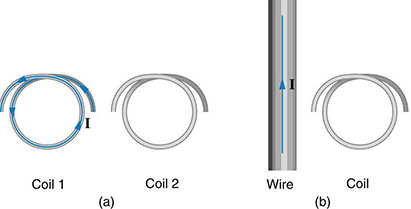
\includegraphics[width=0.4\textwidth]{B-flux.jpeg}
\caption{\label{fig:B-flux} \small (a) A current $I$ flows in the left coil, in the same plane as the right coil. (b) A wire with current $I$ flows in the same plane as the coil.}
\end{figure}
\begin{figure}
\centering
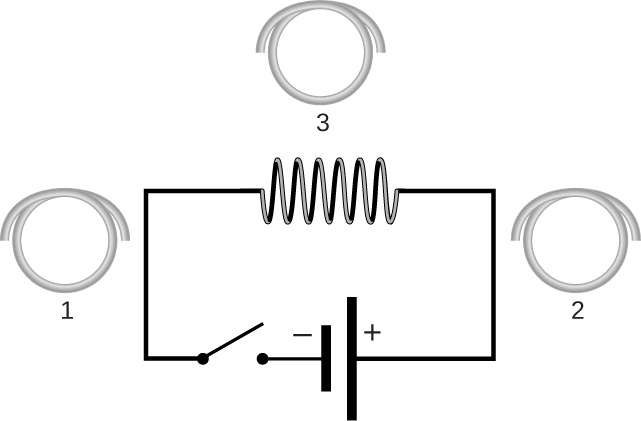
\includegraphics[width=0.4\textwidth]{awesome.jpeg}
\caption{\label{fig:B-flux2} \small A battery provides and emf to a simple circuit with a solenoid, surrounded by three wire loops \textit{in the plane of the circuit}.}
\end{figure}

\noindent
\begin{enumerate}
\item Consider Fig. \ref{fig:B-flux}a.  (a) What is the direction of the current induced in coil 2 if the current in coil 1 increases? If it decreases?  Consider Fig. \ref{fig:B-flux}b.  (b) What is the direction of the current induced in the coil if the current in the wire increases?  If it decreases? \\ \\ \textit{(a) CCW, CW, to oppose changes. (b) CCW, CW, to oppose changes.}
\item Consider Fig. \ref{fig:B-flux2}.  (a) What is the direction of the current induced in coil 1 when the switch is closed?  If it is left closed for a long time?  When it is opened?  (b) Repeat exercise (a) for coil 2.  (c) Repeat exercise (a) for coil 3. \\ \\ \textit{(a) CCW, no current, CW. (b) CCW, no current, CW. (c) No current, no current, no current.}
\item Verify that the units of $\Delta\phi/\Delta t$ are Volts.
\begin{align}
V &= \frac{T m^2}{s} \\
V &= \frac{N A^{-1} m^{-1} m^2}{s} \\
V &= \frac{J m^{-1} A^{-1} m^{-1} m^2}{s} \\
V &= \frac{J A^{-1}}{s} \\
V &= \frac{C V A^{-1}}{s} \\
V &= A V A^{-1} \\
V &= V ~~~ QED
\end{align}
\item (a) An MRI technician moves his hand from a region of very low magnetic field strength into an MRI scanner's 2.00 T field with his fingers pointing in the direction of the field. Find the average emf induced in his wedding ring, given its diameter is 2.20 cm and assuming it takes 0.250 s to move it into the field. (b) What current is induced in the ring if its resistance is 0.0100 $\Omega$?  (c) Calculate the average power dissipated in the ring. \\ \\
\textit{If the fingers are aligned, then assume angle between ring area and B-field is 90 degrees, so $\phi = BA\cos\theta = BA$.  We have}
\begin{align}
\epsilon &= \frac{\Delta \phi}{\Delta t} = \frac{BA}{\Delta t} \\
\epsilon_{\rm ave} &= (\epsilon_{\rm f} + \epsilon_{\rm i})/2 \\
\epsilon_{\rm f} &= (2.0 T \times 2.2\times 10^{-4} m^2)/0.250 s \\
\epsilon_{\rm i} &= 0.0 V \\
\epsilon_{\rm ave} &= 0.5\epsilon_{\rm f} = 0.88 mV
\end{align}
\item Prove that when $B$, $l$, and $v$ are not mutually perpendicular, motional emf is given by $emf = Blv\sin\theta$. If $v$ is perpendicular to $B$, then $\theta$ is the angle between $l$ and $B$. If $l$ is perpendicular to $B$, then $\theta$ is the angle between $v$ and $B$. \textit{Hint: it is helpful to draw a diagram to define the angle $\theta$.} \\ \\
\textit{Treat two cases: (i) $\vec{l}$ is $\perp$ to ${B}$, $\vec{v}$ is not, and (ii) $\vec{v}$ is $\perp$ to ${B}$, $\vec{l}$ is not.  (i) Imagine a uniform $\vec{B}$, with a square loop of wire with area vector aligned with $\vec{B}$.  If the velocity makes an angle $\theta$ with $\vec{B}$, the Faraday's Law says:
\begin{align}
\epsilon &= \frac{\Delta \phi}{\Delta t} = B \frac{\Delta A}{\Delta t} \\
\epsilon &= B l \frac{\Delta x}{\Delta t} = B l v_{\perp} \\
\epsilon &= B l v \sin\theta
\end{align}
In the last step, we use the fact that the only velocity component that changes $A$ is $v\sin\theta$, the component perpendicular to $\vec{B}$.  For case (ii), make the same argument but instead treat only the component of $\vec{B}$ that is perpendicular to $\vec{l}$: $B\sin\theta$.}
\item (a) A bicycle generator rotates at 1875 rad/s, producing an 18.0 V peak emf. It has a 1.00 by 3.00 cm rectangular coil in a 0.640 T field. How many turns are in the coil? (b) What is the period of the AC output of the generator?  \\ \\
\textit{(a) $N = 50$, using $\epsilon_{\rm max} = N B A \omega$. (b) Every 3.35 ms, using $T = 2\pi/\omega$.}
\item An American traveler in New Zealand carries a transformer to convert New Zealand's standard 240 V to 120 V so that she can use some small appliances on her trip. (a) What is the ratio of turns in the primary and secondary coils of her transformer? (b) What is the ratio of input to output current? (c) How could a New Zealander traveling in the United States use this same transformer to power her 240 V appliances from 120 V? \\ \\
\textit{(a) Use $\epsilon_2/\epsilon_1 = N_2/N_1 = 240/120 = 2$. (b) Output current is $1/2$ of input current. (c) Use the transformer in reverse: output becomes input.}
\item Consider Fig. \ref{fig:B-flux2}.  Suppose coil 3 ($N=1$ turn) is rotated 90 degrees such that its normal direction is aligned with the normal direction of the solenoid ($N=6$ turns).  The system is now acting as a \textbf{transformer}.  Suppose the emf in the solenoid is given by $V(t) = V_0 \sin(\omega t)$. (a) Draw a graph of $V(t)$, with the x-axis and y-axis units labeled.  (b) Add the induced emf in coil 3 to your graph, assuming the magnetic flux in coil 3 is rendered identical to that in the solenoid with an iron core.  (c) If $V_0 = 120$ V, and $\omega = (240\pi)$ Hz, when does $V(t) = 0$? \\ \\
\textit{(a) The graph should be a sinusoid, with x-axis labeled with time units, and y-axis labeled with voltage units. (b) If $V(t)$ is a sine wave, then (due to Faradays's Law), coil 3 should have a negative cosine, because the coil responds to \textbf{changes} in $V(t)$.  Also, the amplitude should be smaller.  We do not know the distance between coil 3 and the solenoid, so we cannot say how much smaller. (c) If $\omega = 240\pi$ Hz, then $T = 1/120$ s, so at $t=0$ $V(0) = 0$, and every $1/120$ seconds.}
\item Camera flashes charge a capacitor to high voltage by switching the current through an inductor on and off rapidly. In what time must the 0.100 A current through a 2.00 mH inductor be switched on or off to induce a 500 V emf? \\ \\
\textit{Solve Faraday's Law with inductance for $\Delta t$, which gives $0.4$ $\mu$s.}
\item A large research solenoid has an inductance of 25.0 H. (a) What induced emf opposes shutting it off when 100 A of current through it is switched off in 80.0 ms? (b) How much energy is stored in the inductor at full current? (c) At what rate in watts must energy be dissipated to switch the current off in 80.0 ms? (d) Considering exercise (c), is it surprising that shutting it down this quickly is difficult? (d) Design a solenoid that has an inductance of 25.0 H by choosing the number of turns $N$, the cross-sectional area $A$, and the number of turns $l$. \\ \\
\textit{(a) 31.25 kV. (b) 125 kJ. (c) 1.56 MW. (d) I happened to pick a 5cm radius solenoid that is 50 cm long, with 25.0 H.  This implies $N = 125.8$k turns.  That's a lot of turns, like 2500 turns per cm.  But this is possible with small wire.  The wire must still be thick enough to carry 100.0 A.}
\item Your RL circuit has a characteristic time constant of 20.0 ns, and a resistance of 5.00 M$\Omega$. (a) What is the inductance of the circuit? (b) What resistance would give you a 1.00 ns time constant, perhaps needed for quick response in an oscilloscope? (c) Suppose you design for a 1.00 ns time constant.  What percentage of the final current $I_0$ flows 3.0 ns after the circuit is closed? (d) What is the reactance of the inductor at 10 kHz? \\ \\
\textit{(a) $\tau = L/R$, so $L = R\tau = 5\times 10^6 \times 20 \times 10^{-9} = 0.1$ H. (b) Scaling: 100 M$\Omega$, because a larger resistance gives a smaller time constant. (c) 95\%. (d) $X_{\rm L} = 2\pi f L = 2\pi(10^4)10^{-1} = 2\pi$ k$\Omega$.}
\item An inductor designed to filter high-frequency noise from power supplied to a personal computer is placed in series with the computer. What minimum inductance should it have to produce a 2.00 k$\Omega$ reactance for 15.0 kHz noise? (b) What is its reactance at 60.0 Hz? \\ \\
\textit{(a) Using the formula for inductor reactance, we find $1/(15\pi)$ H, or 21 mH. (b) Using $L = 1/(15\pi)$ H, we find with $f=60$ Hz that $X_L = 8$ $\Omega$.}
\item Consider Fig. \ref{fig:RC}.  Assume the bottom wire is grounded at 0V.  (a) Considering the capacitor reactance, describe why the circuit acts as a \textit{low-pass filter.}  That is, AC signals at $v_{\rm in}$ with \textit{high} frequencies produce very small amplitudes at $v_{\rm out}$. (b) Using Kirchhoff's loop rule on the left side of the circuit, write an equation that describes changes in potential.  (c) Repeat exercise (b) for the right loop.  (d) Solve parts (b) and (c) for $v_{\rm in}$ and $v_{\rm out}$, respectively, and calculate $v_{\rm out}/v_{\rm in}$ in terms of $R$ and $C$.  (e) What is the value of $v_{\rm out}/v_{\rm in}$ for $f = 100(2\pi R C)^{-1}$? For $f = 0.1(2\pi R C)^{-1}$? \\ \\
\textit{(a) For signals with $\omega \gg 1/\tau = 1/RC$, signals at $v_{\rm in}$ feel no resistance from the capacitor, and flow to ground.  Put another way, whatever load is connected to $v_{\rm out}$ will inevitably have a higher resistance or reactance than the capacitor at high frequencies, and will get less of the signal. (b) $v_{\rm in} - iR - i(2\pi fC)^{-1}=0$. (c) $v_{\rm out} - i(2\pi fC)^{-1}=0$.  (d) $v_{\rm out}/v_{\rm in} = 1/(1+2\pi fRC)$.  (e) $0.0099$, and $0.909$, so the lower frequency has the better ratio.}
\begin{figure}
\centering
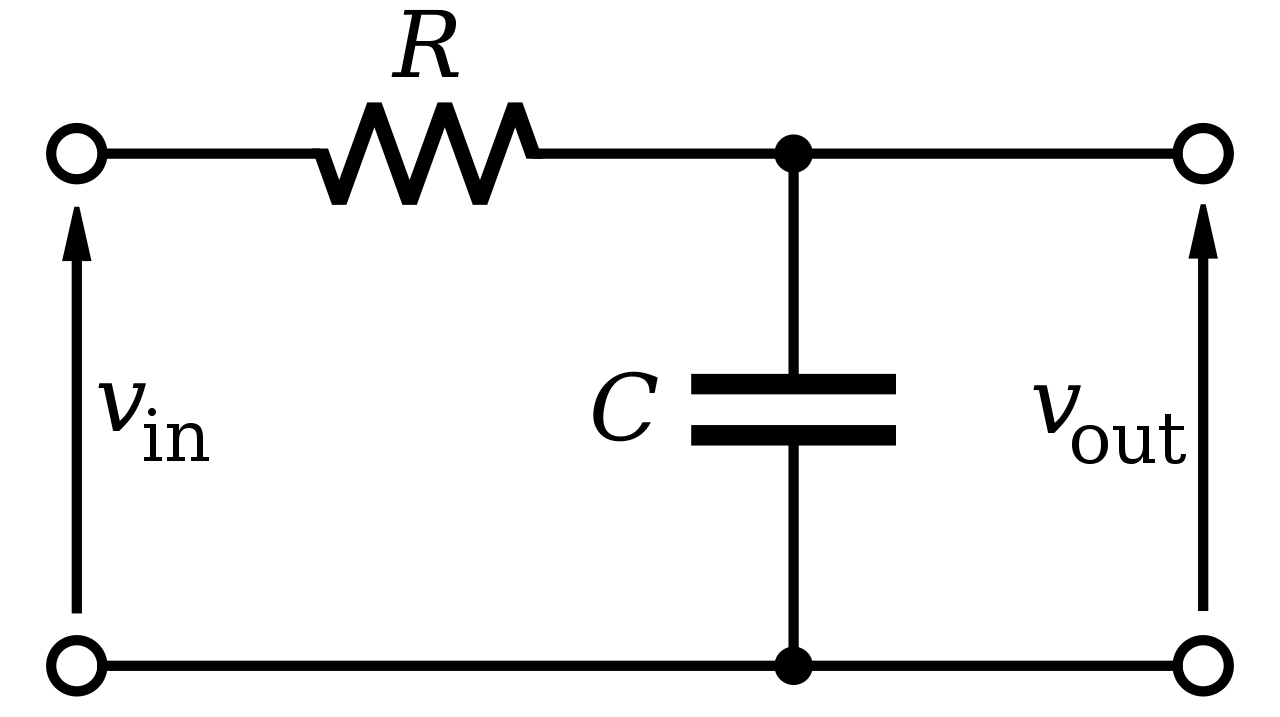
\includegraphics[width=0.25\textwidth]{low-pass.png}
\caption{\label{fig:RC} \small This RC circuit can act as a low-pass filter.}
\end{figure}
\item (a) What are the resonance frequency, $f_0$, and resonance width, $\Delta f/f_0$, of an RLC circuit with $R = 0.1$ k$\Omega$, $C = 1$ $\mu$F, and $L = 10$ mH? (b) What is the total impedance of this circuit at $f = 0.1f_0$ and $f = 10f_0$? \\ \\
\textit{(a) $f_0 = 1/(2\pi)$ MHz, and $\Delta f/f_0 = 1$. (b) For $f = 0.1f_0$, impedance is dominated by the inductor, at about $Z \approx 1.0$ k$\Omega$.  For $f = 10f_0$, the impedance is even more dominated by $X_{\rm L}$: 100 k$\Omega$.}
\item For an RLC circuit with that values of $R$, $L$, and $C$ from the previous problem, and AC source voltage characterized by $V_{\rm rms} = 120$ V, (a) what is $I_{\rm rms}$ at $10 f_0$ and $0.1 f_0$? (b) What is $P_{\rm rms}$ at these frequencies? \textit{Hint: calculate the phase angle between resistance and reactance.} \\ \\
\textit{(a) $I_{\rm rms} = 1.20$ mA, and $120$ mA. (b) For the lower frequency, $\cos\phi = 0.1$, so $P_{\rm ave} = I_{\rm rms} V_{\rm rms}\cos\phi = 120\times 10^{-3} 120 \times 10^{-1}=1.44$ W. For the higher frequency, $\cos\phi = 10^{-3}$, so $P_{\rm ave} = I_{\rm rms} V_{\rm rms}\cos\phi = 1.20\times 10^{-3} 120 \times 10^{-3}=0.144$ mW.}
\item Suppose we are using an LC resonator and diode combination to create an AM radio signal.  If the resonance frequency of our resonator is 1.4 MHz, and our audio signal is at 10 kHz, (a) what three frequencies should be present in our AM radio spectrum?  (b) Suppose our receiver was receiving only the carrier frequency, but not either modulation peak.  Should we gradually increase or gradually decrease the resistance of the receiver circuit?  \\ \\
\textit{(a) 1390, 1400, and 1410 kHz. (b) Gradually increase the resistance until the modulations are received.}
\end{enumerate}

\section{Unit 5: Waves, Optics, Medical Physics}

\begin{figure}[ht]
\centering
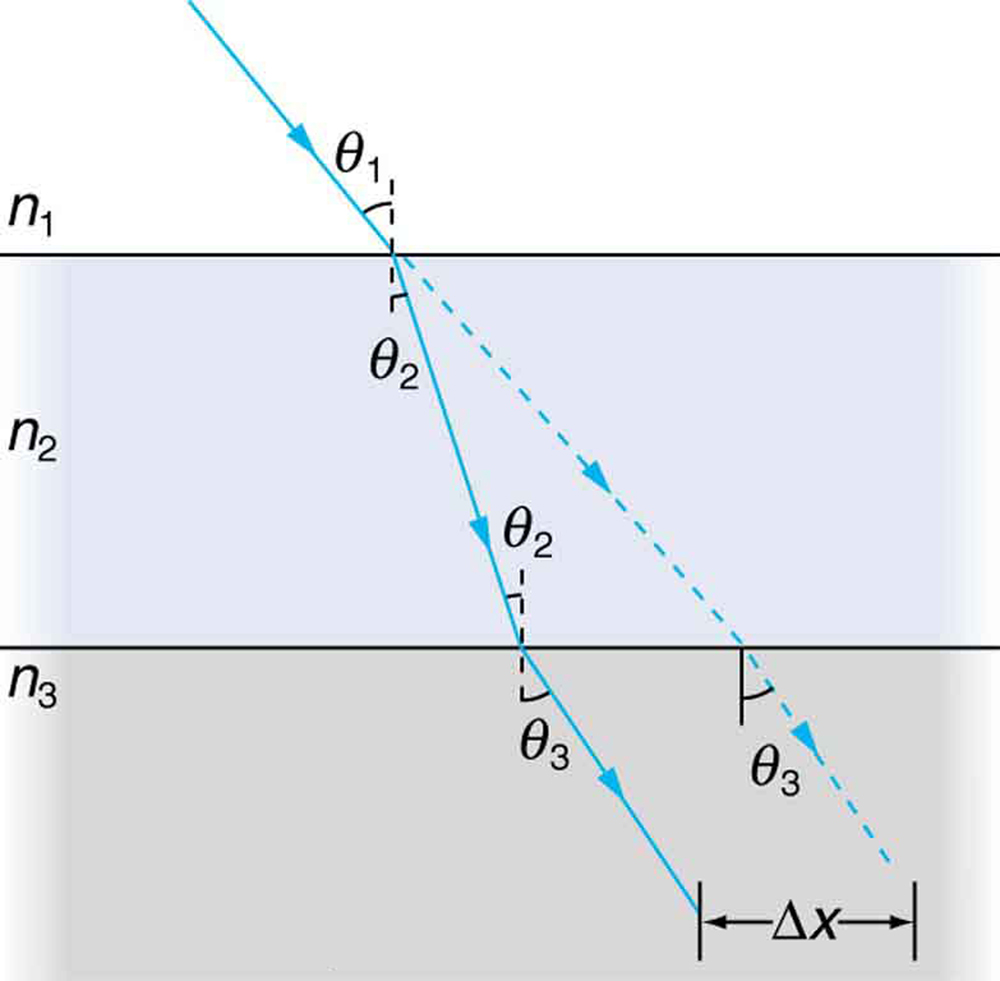
\includegraphics[width=0.25\textwidth]{lens_1.jpeg}
\caption{\label{fig:lens_1} \small A light ray is in a medium with $n_1$, then enters a medium with $n_2$, then a medium with $n_3$.}
\end{figure}

\noindent
\begin{enumerate}
\item (a) What is the B-field generated 0.1 cm laterally from a capacitor in an RC circuit that charges from 0 to 200 nC in 2 $\mu$s? (b) What \textit{current} is responsible for this B-field, since the capacitor is not passing DC current like a wire? \\ \\
\textit{(a) $2$ $\mu$T. (b) The displacement current.}
\item (a) An aircraft receives a pulse reflected from glacial ice below it $10$ $\mu$s after transmission. What is the displacement between aircraft and ice? (b) Suppose the main frequency of the radar is $f = 100$ MHz.  What is the smallest (approximate) change in glacier height the radar operator can observe? (c) What fraction of the radar power is reflected from the ice, assuming normal incidence? \textbf{Bonus.} (d) Suppose the transmitted power at 1 meter is 100 W, and decreases as the inverse of the displacement squared.  What is the received power at the aircraft, accounting for distance and reflection? \\ \\
\textit{(a) 1.5 km. (b) 30 cm. (c) 7.9\%, from the reflection coefficient. (d) $3.5 \times 10^{-6}$, or about -55 dB.}
\item (a) A microwave generates 1 kW of power, projected onto an 10 cm-squared area at a distance of 1 m.  What is the intensity (power per unit area)? (b) How long does it take the energy to travel the 1 meter? (c) What is the peak E-field at the source?  \textbf{Bonus.} (d) If the intensity drops as the distance squared, what is the intensity 2 meters from the microwave?\footnote{Keep in mind that microwaves have protective screens that attenuate this radiation even more than the distance effect does.}\\ \vspace{3cm}
\item Consider Fig. \ref{fig:lens_1}.  (a) Show that $\theta_3 = \theta_1$, if $n_1 = n_3$.  \textit{This proof is the reason why the center of our lenses (like those in our glasses) do not change ray directions.  If our glasses changed the apparent location of objects, they would be useless.} (b) A doctor examines a child's ear with a 15.0 cm focal length magnifying glass held 13.5 cm from the ear. (a) Where is the image? (b) What is its magnification? (c) How big is the image of a 1.0 cm diameter ear hole? \\ \vspace{3cm}
\item (a) What is the ratio of the speed of light in solid ice versus snow?  You may assume fresh snow has the same properties as water for this exercise. (b) If a radio wave transitions from snow to ice with an initial angle of 30 degrees from normal, what is the transmitted angle? \\ \vspace{3cm}
\item (a) Combine thin lens equations to show that the magnification for a thin lens is determined by its focal length and the object distance and is given by $m=f/(f - d_{\rm o})$. (b) Using this equation, determine what conditions lead to $m \to \infty$. (c) What happens to the image location as this condition is met?\footnote{This is why we cannot use lenses to create infinitely large images for free.} \\ \vspace{3cm}
\item Analysis of an interference effect in a clear solid shows that the wavelength of light in the solid is 329 nm. Knowing this light comes from a He-Ne laser and has a wavelength of 633 nm in air, is the substance zircon or diamond? \textit{Maybe this is how they tell if a diamond ring is real ... .}\\ \vspace{1cm}
\item (a) Suppose we are demonstrating the wave-nature of light with a double-slit experiment.  At what angle $\theta$ is the first-order maximum for 400-nm wavelength blue light falling on double slits separated by 0.05 mm? (b) If we double the wavelength to 800 nm, will $\theta$ increase or decrease? (c) Calculate $\theta$ for $\lambda = 800$ nm, $d = 0.05$ mm, and $m = 1$.  \textbf{Bonus.} (d) How would the diffraction pattern change if a glass block with $n = 1.3$ was placed in front of the slits? \\ \vspace{2.5cm}
\item Suppose x-rays have a cross section of 200 barns at 10 keV in a lead vest protecting a medical patient. (a) If the vest is 1 cm thick, what fraction of the x-rays pass through it? (b) At what depth in the vest are half of the x-rays gone? \\ \vspace{2cm}
\item In the previous problem, at what distance would half of the photons be gone if they were $\gamma$ rays insted of x-rays, with a cross section of 1 barn?  \textit{Hint: scaling problem.} \\ \vspace{2cm}
\item \textbf{Bonus.}  The wavelength of an 10 keV x-ray is about 1.2 angstroms, or $1.2 \times 10^{-10}$ m.  (a) What is the momentum of this x-ray? (b) Suppose this x-ray smacks an electron and gives it 50 percent of the momentum.  What is the final speed of the electron, as a fraction of the speed of light? \\ \vspace{2cm}
\item Some nuclear isotopes emit \textit{free neutrons}, neutrons that then propagate outside the nucleus.  These neutrons are useful for controlling nuclear fission for power production, and have a half-life of $611\pm 1$ seconds in free space.  (a) If emitted in free space, what fraction of the neutrons remain after 1 hour? (b) Suppose we start with $10^6$ neutron emitted.  What is the decay \textbf{rate} after 1222 seconds? \\ \vspace{3cm}
\item (a) What is the radioactive dose in rads if 250 mJ of total energy is deposited in the body of a 60 kg adult? (b) What instead would be the dose if the radiation was concentrated in just 2.0 kg of tissue? (c) Assuming the RBE is 1 (x-rays or $\gamma$ rays), what is the dose from part (b) in Sv? (d) Does this dose represent a serious health risk? \\ \vspace{2cm}
\end{enumerate}

\end{document}